\section{Simulation}
To test some \ac{cpp} algorithms is worth to implement an environment which allows to drive a drone autonomously in a safe way, without any risk of collision. PX4 offers different simulators which allow to develop \ac{sitl} simulation \cite{px4_simulation}. More in details, in the section named \textit{MAVROS Offboard control example (Python)} \cite{px4_ros_mavros} there is a useful example on how to setup PX4, Gazebo and MAVROS to run a simulation.

To implement a complete pipeline which allows to develop \ac{cpp} algorithms, simulate the quadcopter and analyse the result MATLAB has been employed beside the simulator structure which exploit PX4, Gazebo and MAVROS, mentioned above. MATLAB is used to determine the area, develop the \ac{cpp} algorithms and pass the waypoint to the simulator. After the simulation phase, which is executed in Gazebo environment the results are visualized and analysed in MATLAB again.

MATLAB is executed in Windows environment, while PX4 software stack, Gazebo and of course \ac{ros} are executed in \ac{wsl} environment (more specifically in Ubuntu 20.04).

\subsection{MATLAB code} 
There are two main files called \texttt{main.m} and \texttt{WSL\_connection.m}; the first one deals with the definition of the target area by the user, the execution of the \ac{cpp} algorithm and consequently the determination of waypoints in space. The second one is devoted to establish the connection with \ac{wsl} to send the waypoint calculated in the \texttt{main.m} file.
\subsubsection*{Main.m code}
As mentioned previously the \texttt{main.m} code is responsible for determining the area of interest and the waypoint calculation.
The first section allows the user to select an area by specifying the latitude and longitude as shown in \ref{fig:target_area_selection}. After the selection procedure the area is converted in local coordinate expressed in meters. This further step is needed because waypoints will be calculated based on robot's footprint.
\lstinputlisting[language=Octave, linerange={5-34}, firstnumber=5]{../simulator/main.m}
\begin{figure}[hbt!]
	\centering
	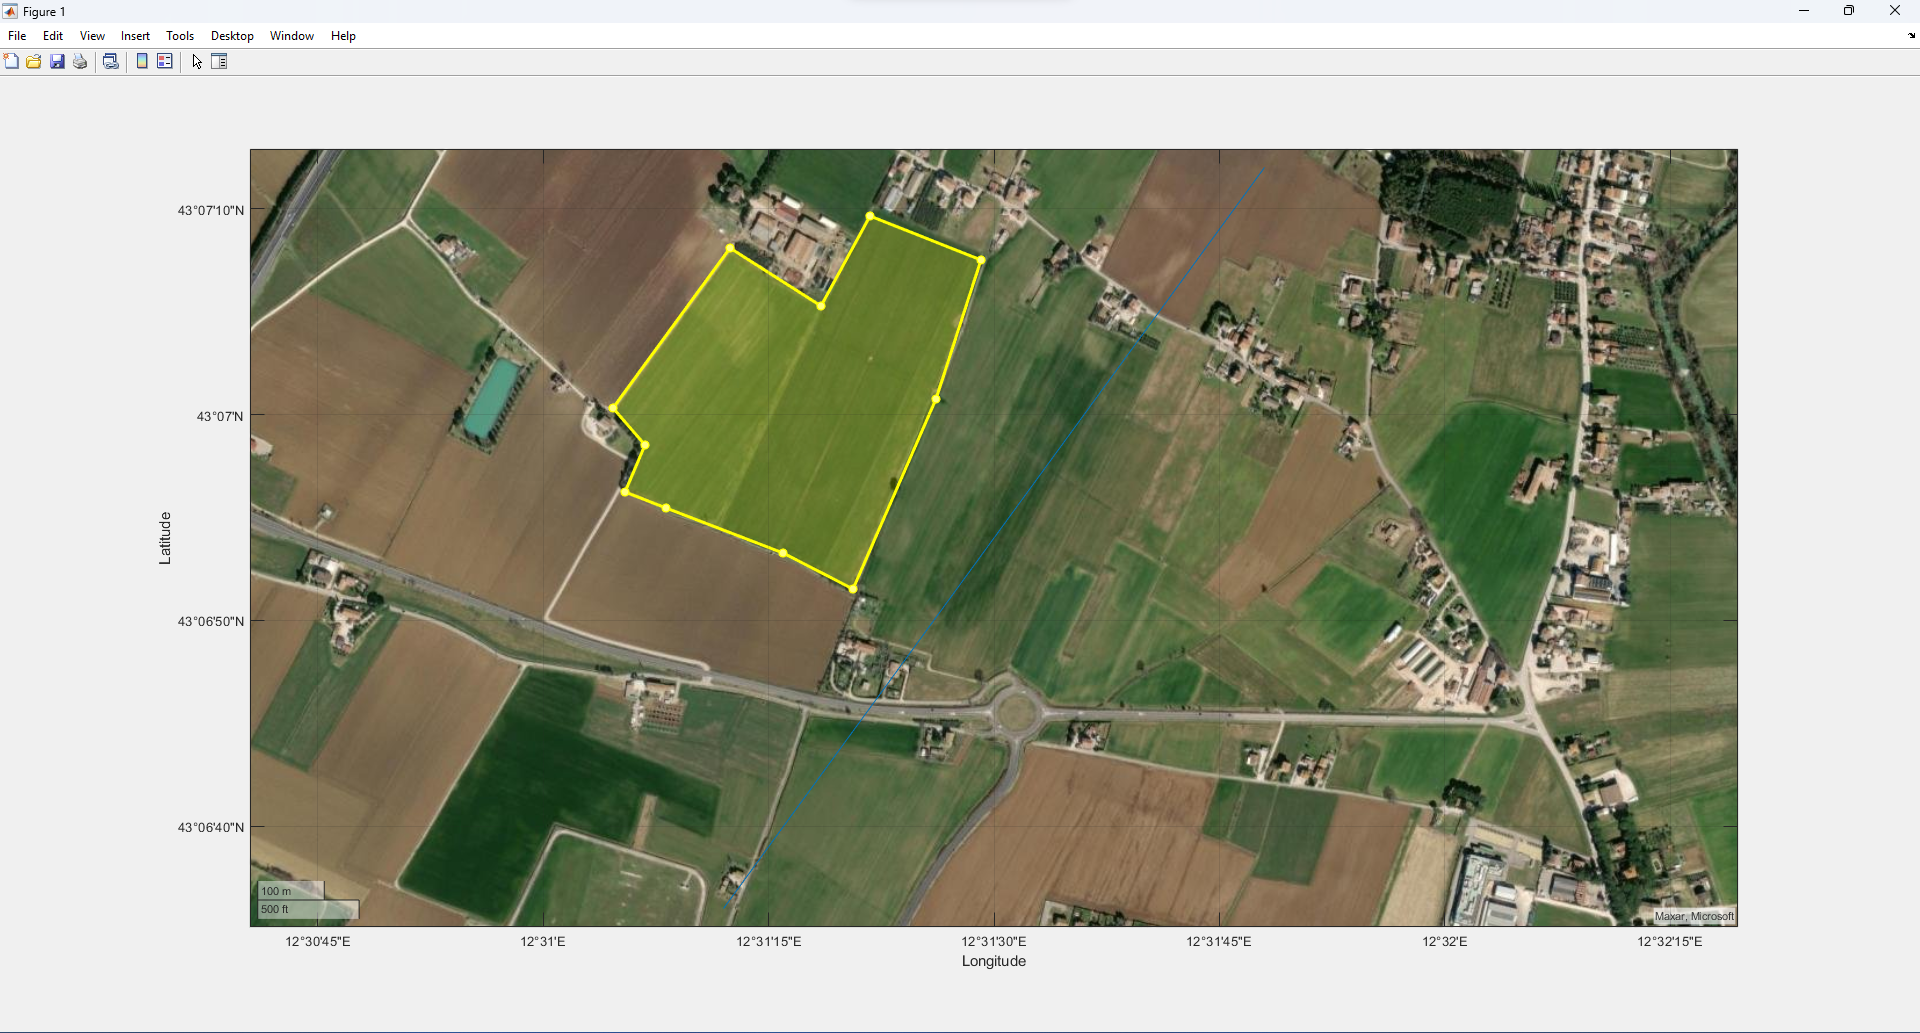
\includegraphics[width=\linewidth]{images/target_area_selection}
	\caption{Target area selection.}
	\label{fig:target_area_selection}
\end{figure}

The next section is devoted to the application of the \ac{cpp} algorithm to the selected area, it returns a 2D or 3D waypoints, these last ones will be passed to the simulator through the \texttt{WSL\_connection.m} file.
\lstinputlisting[language=Octave, linerange={39-74}, firstnumber=39]{../simulator/main.m}

\subsection*{WSL\_connection.m code}
This script is responsible for the connection with \ac{wsl}, which means that allows MATLAB to interact with the rostopic executed on \ac{wsl}, it automatically recovers the ip addresses needed
\footnote{This code is tested in Windows system, to recover the addresses through Windows terminal and ubuntu shell type the following commands: 
\begin{itemize}
	\item In Ubuntu shell type \texttt{\$ ifconfig} and look for the address named \texttt{iner} under \texttt{eth0}. This is the variable named \texttt{ipAdd\_wsl}.
	\item In Windows terminal type \texttt{\$ ip config} and look for \texttt{IPv4 address} under \texttt{Ethernet Card vEthernet (WSL). This is the variable named \texttt{ipAdd\_Windows}}.
\end{itemize}}.
\lstinputlisting[language=Octave, linerange={1-23}, firstnumber=1]{../simulator/WSL_connection.m}

In addition, the second section is responsible of instantiating a new node which publish the waypoint list\footnote{The code assumes that there is a matrix variable named \texttt{waypoint3D}, wtih dimensions $N \times 3$, where $N$ represents the number of waypoint and the columns are the $xyz$ coordinates in the space.} in the topic named \texttt{/MATLAB\_waypoint}.
\lstinputlisting[language=Octave, linerange={26-47}, firstnumber=26]{../simulator/WSL_connection.m}

\subsection{WSL environment}
\ac{wsl} is used to run the simulations, it exploits the PX4 autopilot with Gazebo and MAVROS. First of all the following components need to be installed:
\begin{itemize}
	\item PX4 autopitlot folder, downloadable by following the section named \href{https://docs.px4.io/main/en/dev_setup/dev_env_linux_ubuntu.html}{\textit{Ubuntu Development Environment}}. 
	\item \ac{ros} and MAVROS\footnote{The installation of \ac{ros} and MAVROS is not covered in this guide.}
\end{itemize}
The idea behind the simulation is to use MAVROS to drive in off-board mode a simulated quadcopter in Gazebo using the waypoint calculated in MATLAB. As a result, we need a ac{ros} that is capable of subscribing to the topic named \texttt{/MATLAB\_waypoint} to recover the waypoint list. By following PX4 documentation sections named \href{https://docs.px4.io/main/en/ros/mavros_offboard_python.html}{\textit{MAVROS Offboard control example (Python)
}} is easy to understand how to develop a new \ac{ros} package\footnote{\texttt{catkin\_make} can be used instead of\texttt{catkin build}, for more details take a look at ROS documentation section named \href{http://wiki.ros.org/ROS/Tutorials/CreatingPackage}{\textit{Creating a ROS Package}.
}}.
The file implemented to create the rosnode is called \texttt{waypoint\_manager.py}. 

\subsubsection*{Waypoint\_manager.py}
The code should be easily readable by the user, for more details contact the author. %TODO explain the code 
 % the code is written in lstlisting env beacause is not possible to link it since it lies in WSL
\begin{lstlisting}[language=Python]
	#!/usr/bin/env python3
	
	import rospy
	from geometry_msgs.msg import PoseStamped, Point, PoseArray
	from mavros_msgs.msg import State
	from mavros_msgs.srv import CommandBool, CommandBoolRequest, SetMode, SetModeRequest
	from math import dist
	
	
	current_state = State()
	
	waypoint_index = 0
	waypointList = []
	waypointReceived = False # flag to check if waypoint list is received
	nextWaypoint = [0, 0, 0]
	
	
	
	def state_cb(msg):
		global current_state
		current_state = msg
	
	
	def buildWPArray(data):
		for index in range(len(data.poses)):
		waypointList.append([data.poses[index].position.x, data.poses[index].position.y, data.poses[index].position.z])
	
	
	def getNextWP(currentPosition, threshold):
	
		global waypoint_index
		global waypointList
		global nextWaypoint
	
		try: 
			currentWaypoint = waypointList[waypoint_index]
			nextWaypoint = currentWaypoint
			
			if dist(currentPosition, currentWaypoint) < threshold: # compute euclidean 3D distance
			waypoint_index += 1
			nextWaypoint = waypointList[waypoint_index]
			rospy.loginfo('Next waypoint: ' + str(nextWaypoint))             
	
		except IndexError:
			pass
	
	
	return nextWaypoint
	
	
	
	def WP_callback(data):
	
		if waypointReceived:
		
		targetWP = getNextWP([data.pose.position.x,
		data.pose.position.y,
		data.pose.position.z], threshold=.2)          
		
		
		
		# Create a PoseStamped message
		pose_msg = PoseStamped()
		pose_msg.header.stamp = rospy.Time.now()
		pose_msg.pose.position.x = targetWP[0]
		pose_msg.pose.position.y = targetWP[1]
		pose_msg.pose.position.z = targetWP[2]
		pose_msg.pose.orientation.x = 0.0
		pose_msg.pose.orientation.y = 0.0
		pose_msg.pose.orientation.z = 0.0
		pose_msg.pose.orientation.w = 0.0
		
		currentWaypoint_pub.publish(pose_msg)
		
		#else:
		#    rospy.loginfo('Waiting for waypoint')
	
	if __name__ == '__main__':
	
		try:
		
		rospy.init_node('waypoint_manager')
		
		# subscribers
		state_sub = rospy.Subscriber("mavros/state", State, callback = state_cb)
		position_sub = rospy.Subscriber('mavros/local_position/pose', PoseStamped, callback = WP_callback)
		
		# publisher
		currentWaypoint_pub = rospy.Publisher('/mavros/setpoint_position/local', PoseStamped, queue_size=10)
		
		
		rospy.wait_for_service("/mavros/cmd/arming")
		arming_client = rospy.ServiceProxy("mavros/cmd/arming", CommandBool) 
		
		rospy.wait_for_service("/mavros/set_mode")
		set_mode_client = rospy.ServiceProxy("mavros/set_mode", SetMode)
		
		waypointMessage = rospy.wait_for_message("/MATLAB_waypoint", PoseArray)
		buildWPArray(waypointMessage)
		rospy.loginfo("Waypoint list: " + str(waypointList))
		waypointReceived = True    
	
	
		# Setpoint publishing MUST be faster than 2Hz
		rate = rospy.Rate(20)
		
		# Wait for Flight Controller connection
		while(not rospy.is_shutdown() and not current_state.connected):
			rate.sleep()
	
		offb_set_mode = SetModeRequest()
		offb_set_mode.custom_mode = 'OFFBOARD'
	
		arm_cmd = CommandBoolRequest()
		arm_cmd.value = True
		
		last_req = rospy.Time.now()
	
		while(not rospy.is_shutdown()):
			if(current_state.mode != "OFFBOARD" and (rospy.Time.now() - last_req) > rospy.Duration(5.0)):
				if(set_mode_client.call(offb_set_mode).mode_sent == True):
					rospy.loginfo("OFFBOARD enabled")
	
				last_req = rospy.Time.now()
				
			else:
				if(not current_state.armed and (rospy.Time.now() - last_req) > rospy.Duration(5.0)):
					if(arming_client.call(arm_cmd).success == True):
						rospy.loginfo("Vehicle armed")	
						
					last_req = rospy.Time.now()
	
			rate.sleep()
	
		rospy.spin()
	
	except rospy.ROSInterruptException:
		rospy.logwarn("Node Interrupted")
\end{lstlisting}

\subsection{Execute simulation}
Is recommendable to don't use a \texttt{.launch}, launch all the files from different terminal. These are the steps to successfully run the simulation:
\begin{enumerate}
	\item Run \texttt{main.m} file to calculate the waypoints
	\item On the first terminal run the command \texttt{\$ roslaunch PX4-Autopilot/launch/mavros\_posix\_sitl.launch} to launch the PX4 autopoilot and Gazebo environment
	\item On the second terminal run the command \\
	\texttt{\$ rosrun offboard\_py waypoint\_manager.py} to launch the \texttt{waypoint\_manager} node
	\item Run \texttt{WSL\_connection.m} to send the waypoint list to the \texttt{waypoint\_manager} node
\end{enumerate}
After this the situation should look like the one depicted in Figure \ref{fig:rqt_graph_view}.
\begin{figure}[hbt!]
	\centering
	\includegraphics[width=\linewidth]{"images/rqt_graph view"}
	\caption{Node and topic view focused on \texttt{waypoint\_manager} node.}
	\label{fig:rqt_graph_view}
\end{figure}
